\documentclass[t]{beamer}
\mode<presentation>

\usepackage{etex}

\usetheme{Madrid}
% other themes: Warsaw, AnnArbor, Antibes, Bergen, Berkeley, Berlin, Boadilla, boxes, CambridgeUS, Copenhagen, Darmstadt, default, Dresden, Frankfurt, Goettingen,
% Hannover, Ilmenau, JuanLesPins, Luebeck, Madrid, Maloe, Marburg, Montpellier, PaloAlto, Pittsburg, Rochester, Singapore, Szeged, classic

\setbeamertemplate{navigation symbols}{\insertslidenavigationsymbol}

\usecolortheme{dolphin}
%\usecolortheme{seagull}
% color themes: albatross, beaver, beetle, crane, default, dolphin, dov, fly, lily, orchid, rose, seagull, seahorse, sidebartab, structure, whale, wolverine

%\usefonttheme{serif}
% font themes: default, professionalfonts, serif, structurebold, structureitalicserif, structuresmallcapsserif

% pdf is displayed in full screen mode automatically
%\hypersetup{pdfpagemode=FullScreen}

%\AtBeginSection[]
%{
%  \begin{frame}<beamer>
%    \frametitle{Outline}
%    \tableofcontents[currentsection,currentsubsection]
%  \end{frame}
%}

% define your own colours:
\definecolor{Red}{rgb}{1,0,0}
\definecolor{Blue}{rgb}{0,0,1}
\definecolor{Green}{rgb}{0,1,0}
\definecolor{magenta}{rgb}{1,0,.6}
\definecolor{lightblue}{rgb}{0,.8,1}
\definecolor{lightpurple}{rgb}{.6,.4,1}
\definecolor{gold}{rgb}{.6,.5,0}
\definecolor{orange}{rgb}{1,0.4,0}
\definecolor{hotpink}{rgb}{1,0,0.5}
\definecolor{newcolor2}{rgb}{.5,.3,.5}
\definecolor{newcolor}{rgb}{0,.3,1}
\definecolor{newcolor3}{rgb}{1,0,.35}
\definecolor{darkgreen1}{rgb}{0, .35, 0}
\definecolor{darkgreen}{rgb}{0, .6, 0}
\definecolor{darkred}{rgb}{.75,0,0}

\xdefinecolor{olive}{cmyk}{0.64,0,0.95,0.4}
\xdefinecolor{purpleish}{cmyk}{0.75,0.75,0,0}

%\usepackage{beamerinnerthemerounded}
% inner themes include circles, default, inmargin, rectangles, rounded

%\usepackage{beamerouterthemesmoothbars}
% outer themes include default, infolines, miniframes, shadow, sidebar, smoothbars, smoothtree, split, tree

\useoutertheme[subsection=false]{smoothbars}

% to have the same footer on all slides
\setbeamertemplate{footline}[text line]{
\raisebox{3pt}{
\includegraphics[height=15pt]{su-long.eps}}\hfill 
\raisebox{5pt}{Math 207:  Statistics}\hfill 
\raisebox{5pt}{The Accuracy of Averages}\hfill
\raisebox{5pt}{\insertframenumber/\pageref{lastpage}}}
%\setbeamertemplate{footline}[text line]{} % or empty footer

% include packages
\usepackage{subfigure}
\usepackage{multicol}
\usepackage{amsmath}
\usepackage{epsfig}
\usepackage{graphicx}
\usepackage[all,knot]{xy}
\xyoption{arc}
\usepackage{url}
\usepackage{multimedia}
\usepackage{hyperref}
\usepackage{setspace}

\title{Math 207:  Statistics}
\subtitle{Chapter 23:  The Accuracy of Averages}
\author{Ralph Wojtowicz}
\institute{Mathematics Department\\ Shenandoah University}
%\date{\scriptsize 17 February 2012}

\usepackage{pstricks,pst-grad,pst-func,pst-text,pst-node,multido,pst-plot,calc,pst-3dplot}

\newcommand{\BRACE}{
\begin{pspicture}(-3,-2.1)(3,1.1)
\psset{yunit=3,linewidth=0.02}
\psline(-3.5,0)(3.5,0)  
  \psline(-3,0)(-3,-0.04) \rput[t](-3,-0.07){\scriptsize -3\hphantom{-}}
  \psline(-2,0)(-2,-0.04) \rput[t](-2,-0.07){\scriptsize -2\hphantom{-}}
  \psline(-1,0)(-1,-0.04) \rput[t](-1,-0.07){\scriptsize -1\hphantom{-}}
  \psline(0,0)(0,-0.04)   \rput[t](0,-0.07){\scriptsize 0}
  \psline(1,0)(1,-0.04)   \rput[t](1,-0.07){\scriptsize 1}
  \psline(2,0)(2,-0.04)   \rput[t](2,-0.07){\scriptsize 2}
  \psline(3,0)(3,-0.04)   \rput[t](3,-0.07){\scriptsize 3}
  \rput[l](3.6,0){\scriptsize $x$}
\psline(0,0)(0,0.5)
  \psline(-0.12,0.5)(0,0.5)    \rput[r](-0.21,0.5){\scriptsize $0.5$}
  \psline(-0.12,0.25)(0,0.25)  \rput[r](-0.21,0.25){\scriptsize $0.25$}
\psGauss[linecolor=blue,linewidth=0.02,sigma=1,mue=0]{-3}{3}
\pnode(-1,-0.15){A}\pnode(1,-0.15){B}
\psbrace[braceWidth=0.02,braceWidthInner=5pt,braceWidthOuter=5pt](A)(B){\rput{90}(0.25,-0.05){\scriptsize 68\%}}
%
\pnode(-2,-0.15){C}\pnode(2,-0.15){D}
\psbrace[braceWidth=0.02,braceWidthInner=25pt,braceWidthOuter=5pt](C)(D){\rput{90}(0.25,-0.05){\scriptsize 95\%}}
%
\pnode(-3,-0.15){E}\pnode(3,-0.15){F}
\psbrace[braceWidth=0.02,braceWidthInner=45pt,braceWidthOuter=5pt](E)(F){\rput{90}(0.25,-0.1){\scriptsize 99.7\%}}
\end{pspicture}}

\begin{document}

%\frame[plain]{
%	\titlepage
%}


\begin{frame}[plain]
\definecolor{myblue}{rgb}{0,0,0.6}
\definecolor{grayA}{rgb}{0.95,0.95,0.95}
\definecolor{grayB}{rgb}{0.98,0.98,0.98}
\begin{center}

%\begin{pspicture}(0,0)(7,4.8)
\begin{pspicture}(-6,-7)(6,2)

%\rput(0,-1.85){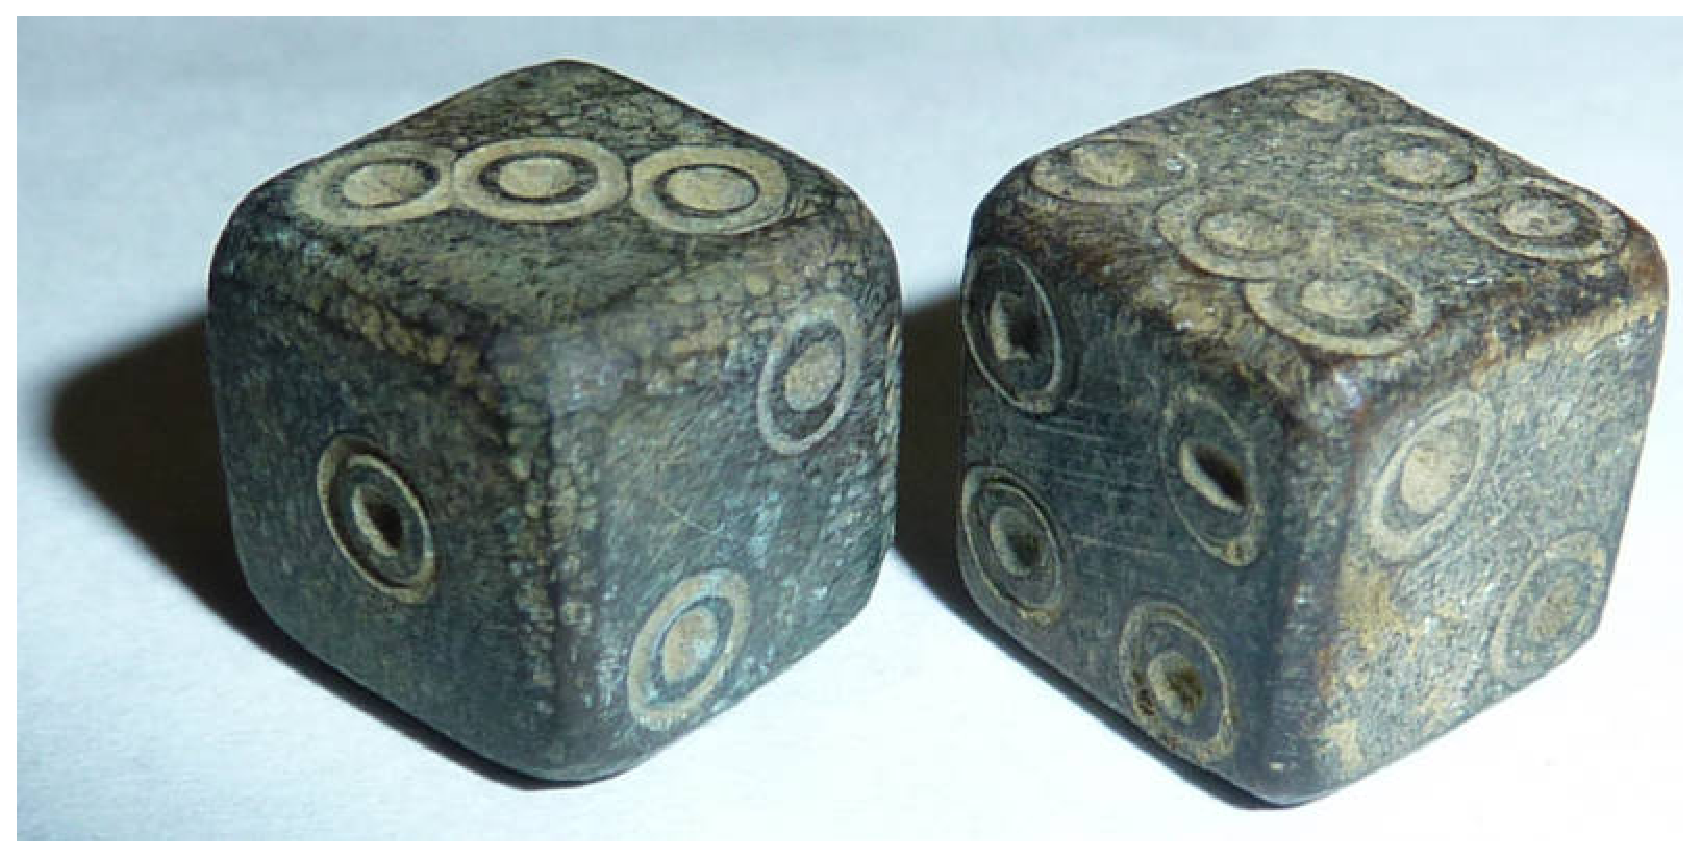
\includegraphics[height=4.2cm]{dice.eps}}
\psframe[linewidth=0.02,linecolor=gray](-6.2,-7)(6.2,2.2)
\psframe[linewidth=0.02,linecolor=gray](-6.15,-6.95)(6.15,2.15)
\rput(0,1.4){\color{myblue}\large Math 207:  Statistics}
\rput(0,0.6){\color{myblue}Chapter 23: The Accuracy of Averages}
%
\psframe[linewidth=0.02,fillstyle=solid,fillcolor=grayA](-2,-3)(2,-1)
  \rput[tl](-1.9,-1.1){\tiny Population (parameters)}
\psframe[linewidth=0.02,fillstyle=solid,fillcolor=grayB](-0.25,-2.75)(1.75,-2)
  \rput[tl](-0.15,-2.1){\tiny Sample (statistics)}
%\psframebox(0,0)(4,4)
\rput(0,-4.5){\scriptsize Dr.~Ralph Wojtowicz}
\rput(0,-5.0){\scriptsize Mathematics Department}
\rput(0,-5.8){
\includegraphics[height=1cm]{su-long.eps}}
%
%\rput(0,-6.5){\scriptsize 17 February 2012}
\end{pspicture}
\end{center}

\end{frame}

%\section[Outline]{}

\addtocounter{page}{-1}
\addtocounter{framenumber}{-1}

{\footnotesize
\frame{\tableofcontents}
}

\section{EV, SE and the Central Limit Theorem}

\begin{frame}
\frametitle{Expected Value, Standard Error,  Central Limit Theorem}
\begin{center}

\footnotesize

\begin{itemize}
\item Many statistics problems are modeled as  samples
   from a box of numbered tickets.
\item Solution procedure: 
   \begin{itemize}
   \item \scriptsize Formulate a box model.
   \item \scriptsize Compute the average and SD of the contents of the box.
   \item \scriptsize Determine if you are computing a sum or average (\%
      in a 0/1 box is an average).
   \item Use the appropriate formulas to compute the EV and SE
      for the sample.
   \item Use the normal curve  to compute chances of the 
      sample being in a specified range.
   \end{itemize}
\end{itemize}
%\begin{pspicture}(0,0)(7,4.8)
\begin{pspicture}(-6,-7)(6,0.2)
\rput(0.8, -1.4){
\begin{tabular}{cc}
\scalebox{0.65}{\begin{pspicture}(1.2,0)(11.3,4)
\psset{yunit=0.05, xunit=2.25}
\psline[linestyle=dotted](1,0)(4,0)
\rput[t](2.5,80){\textbf{Sum of Draws}}
\rput(2.5,65){$\mbox{EV}_{\mbox{\scriptsize sum}} = n\times\mbox{AV}_{\mbox{\scriptsize box}}$}
\rput(2.56,55){$\mbox{SE}_{\mbox{\scriptsize sum}} = \sqrt{n}\times\mbox{sd}_{\mbox{\scriptsize box}}$}
\psline(1.000000, -1)(1.301030, 0)(1.477121, 2)(1.602060, 1)(1.698970, 0)(1.778151, -1)(1.845098, -3)(1.903090, -5)(1.954243, -5)(2.000000, -6)(2.301030, -2)(2.477121, -4)(2.602060, -1)(2.698970,  5)(2.778151, 12)(2.845098, 18)(2.903090, 13)(2.954243, 8)(3.000000, 2)(3.301030, 13)(3.477121, 10)(3.602060, 29)(3.698970, 33)(3.778151, 9)(3.845098, 16)(3.903090, 34)(3.954243, 38)(4.000000, 67)
\psset{linewidth=0.02}
%
\psline(1,-20)(0.95,-20)\rput[r](0.92,-20){-20}
\psline(1,0)(0.95,0)    \rput[r](0.92,0){0}
\psline(1,20)(0.95,20)  \rput[r](0.92,20){20}
\psline(1,40)(0.95,40)  \rput[r](0.92,40){40}
\psline(1,60)(0.95,60)  \rput[r](0.92,60){60}
\psline(1,80)(0.95,80)  \rput[r](0.92,80){80}
\psline(1,-20)(1,80) % y axis
\rput{90}(0.4,30){Number of Heads Minus}
\rput{90}(0.6,30){Half the Number of Tosses}
%
\psline(1,-20)(1,-24)\rput[t](1,-26){10}
\psline(2,-20)(2,-24)\rput[t](2,-26){100}
\psline(3,-20)(3,-24)\rput[t](3,-26){1,000}
\psline(4,-20)(4,-24)\rput[t](4,-26){10,000}
\psline(1,-20)(4,-20) % x axis
\rput(2.5,-40){Number of Tosses}
\end{pspicture}}
&
\scalebox{0.65}{\begin{pspicture}(3,0)(12,4)
\psset{yunit=0.05, xunit=2.25}
\psline[linestyle=dotted](1,30)(4,30)
\rput[t](2.5,80){\textbf{Percent of Draws}}
\rput(2.5,65){$\mbox{EV}_{\mbox{\scriptsize av}} = \mbox{AV}_{\mbox{\scriptsize box}}$}
\rput(2.65,55){$\mbox{SE}_{\mbox{\scriptsize av}} = \mbox{sd}_{\mbox{\scriptsize box}}\,/\sqrt{n}$}
\psline(1.000000, -20)(1.301030, 30)(1.477121, 63.3)(1.602060, 42.5)(1.698970, 30)(1.778151, 21.67)(1.845098, 8.57)(1.903090, -1.25)(1.954243, 2.22)(2.000000, 0)(2.301030, 25)(2.477121, 23.3)(2.602060, 28.75)(2.698970,  35)(2.778151, 40)(2.845098, 42.86)(2.903090, 38.125)(2.954243, 34.44)(3.000000, 31)(3.301030, 33.25)(3.477121, 31.67)(3.602060, 33.625)(3.698970, 33.3)(3.778151, 30.75)(3.845098, 31.14)(3.903090, 32.125)(3.954243, 32.111)(4.000000, 33.35)
\psset{linewidth=0.02}
%
\psline(1,-20)(0.95,-20)\rput[r](0.92,-20){-10}
%\psline(1,0)(0.95,0)    \rput[r](0.92,0){0}
\psline(1,5)(0.95,5)  \rput[r](0.92,5){-5}
\psline(1,30)(0.95,30)  \rput[r](0.92,30){0}
\psline(1,55)(0.95,55)  \rput[r](0.92,55){5}
\psline(1,80)(0.95,80)  \rput[r](0.92,80){10}
\psline(1,-20)(1,80) % y axis
%\rput{90}(0.45,30){Number of Heads Minus}
\rput{90}(0.6,30){Percentage of Heads $-$ 50\%}
%
\psline(1,-20)(1,-24)\rput[t](1,-26){10}
\psline(2,-20)(2,-24)\rput[t](2,-26){100}
\psline(3,-20)(3,-24)\rput[t](3,-26){1,000}
\psline(4,-20)(4,-24)\rput[t](4,-26){10,000}
\psline(1,-20)(4,-20) % x axis
\rput(2.5,-40){Number of Tosses}
\end{pspicture}}
\end{tabular}}
\end{pspicture}
\end{center}

\end{frame}

\section{Examples}
\subsection{Example I}
\begin{frame}
\frametitle{Example:  Box Contents Known}

\footnotesize

\begin{itemize}
\item<2-> Take a random sample of size $n=100$ from the box below.
\begin{center}
\scalebox{0.8}{\psframebox{\psframebox{1}\;\psframebox{2}\;\psframebox{3}\;\psframebox{4}\;%
         \psframebox{5}\;\psframebox{6}\;\psframebox{7}}}
\end{center}
\item<3-> $\mbox{AV}_{\mbox{\scriptsize box}}=\frac{1+2+\cdots + 7}{7} =4$
and $\mbox{SD}_{\mbox{\scriptsize box}}=\sqrt{\frac{(1-4)^2+(2-4)^2+\cdots + (7-4)^2}{7}}=\sqrt{\frac{28}{7}}=\sqrt{4}=2$.
\item<4-> $\mbox{EV}_{\mbox{\scriptsize av}}=\mbox{AV}_{\mbox{\scriptsize box}}=4$
 and $\mbox{SE}_{\mbox{\scriptsize av}}=
    \frac{\footnotesize\mbox{\scriptsize SD}_{\mbox{\tiny box}}}{\sqrt{n}}\approx 
    \frac{4}{\sqrt{100}} = 0.4$.
\item<5-> We expect the average of the draws to be around 4 give or take $0.4$ or so.
\item<6-> What is the chance that the average will be between $3.5$ and $4.5$?
\item<7-> Compute the $z$ scores for 61\% and 65\%:\\
   $z_1=(3.5 - 4)/0.4 = -1.25$\\[2pt]
   $z_2=(4.5 - 4)/0.4 = 1.25$\\
\item<8->  Area under the normal curve:~{\scriptsize $\mbox{\texttt{pnorm}}(1.25) - \mbox{\texttt{pnorm}}(-1.25) = 
   0.789=78.9\%$}
\end{itemize}

\end{frame}


\subsection{Example I}
\begin{frame}
\frametitle{Example:  Box Contents Unknown}

\footnotesize

\begin{itemize}
\item<2-> Take a random sample of size $n=100$ from the box below.\vspace{-2pt}
\begin{center}
\scalebox{0.8}{\psframebox{\psframebox{?}\hspace{5pt}$\cdots$\hspace{5pt}\psframebox{?}}}
\end{center}
We don't know what numbers are in the box!
\item<3->  Suppose our sample of size 100 has an average of $10.2$ and an SD of $0.8$.  
\item<4->  Estimate the true average of the tickets to be $10.2$ but also give  a plus or minus on the 
    estimate.
\item<5->  {\color{blue}Estimate} $\mbox{SD}_{\mbox{\scriptsize box}}=0.8$.
\item<5-> 
  $\mbox{SE}_{\mbox{\scriptsize av}}=
    \frac{\scriptsize\mbox{SD}_{\mbox{\tiny box}}}{\sqrt{n}}\approx 
    \frac{0.8}{\sqrt{100}} = 0.08$.
\item<6-> If we assume that the samples follow a normal curve, then 
\[10.2\; \pm\; 2\cdot (0.08) = 10.2\; \pm 0.16\]
is {\color{blue}95\% confidence interval} on the average of the box.
\end{itemize}

\end{frame}

\section{Confidence Intervals}
\subsection{Inferential Statistics}
\begin{frame}
\frametitle{Inferential Statistics}

\footnotesize
\begin{itemize}
\item In real situations, we typically don't know the contents of the box!
\item That is where {\color{blue}inferential statistics} is used.
\end{itemize}

\begin{center}
{\begin{pspicture}(0,-1.1)(3,4.2)
\psset{linewidth=0.02}
\rput(1.5,4){\rnode{Statistics}{\psframebox{Statistics}}}
\pnode(1.5,3){NULL}
\rput(-1,3){\ovalnode{Descriptive}{\hspace{-12pt}
    \begin{tabular}{c}Descriptive\\ Statistics\end{tabular}\hspace{-12pt}}}
\rput(4,3){\ovalnode{Inferential}{\hspace{-8pt}\begin{tabular}{c}Inferential\\ Statistics\end{tabular}\hspace{-8pt}}}
\rput[t](-1,1.5){\rnode{ID}{\psframebox{\hspace{-4pt}\begin{tabular}{l}Includes\\ 
        $\bullet$ Collecting,\\ 
        $\bullet$ Organizing, \\ 
        $\bullet$ Summarizing and\\ 
        $\bullet$ Presenting\\ 
        \hphantom{$\bullet$ }{data}\end{tabular}\hspace{-4pt}}}}
\rput[t](4,1.5){\rnode{II}{\psframebox{\hspace{-4pt}\begin{tabular}{l}Includes\\ 
        $\bullet$ Making inferences,\\ 
        $\bullet$ Hypothesis testing,\\ 
        $\bullet$ Determining \\ \hphantom{$\bullet$} relationships and\\ 
        $\bullet$ Making predictions\\ \end{tabular}\hspace{-4pt}}}}
\psset{linewidth=0.04}
\ncline{->}{Statistics}{NULL}
\ncline{->}{NULL}{Descriptive}
\ncline{->}{NULL}{Inferential}
\ncline{->}{Descriptive}{ID}
\ncline{->}{Inferential}{II}
\end{pspicture}}
\end{center}

\end{frame}

\subsection{Confidence Intervals}
\begin{frame}
\frametitle{Confidence Intervals}

\footnotesize
\begin{itemize}
\item In real situations, we typically don't know the contents of the box!
\item<2-> We can take a sample and  compute a {\color{blue}confidence 
   interval} on the average of the numbers in the box.
\item<3-> This gives an estimate of the average and puts a plus-or-minus on the estimate.
\vspace{-10pt}
\end{itemize}

\uncover<3->{\[\mbox{EV}_{\mbox{\scriptsize av}} =  \mbox{AV}_{\mbox{\scriptsize box}}\hspace{20pt}
\mbox{SE}_{\mbox{\scriptsize av}} = 
  \frac{\mbox{SD}_{\mbox{\tiny box}}}{\sqrt{n}}\vspace{-5pt}\]}

\begin{itemize}
\item<5-> Take a random sample of size $n$.
\item<6-> Compute the average and SD of the sample.
\item<7-> Use the SD of the sample to approximate the SD of the box.
\item<8-> Then compute the $\mbox{SE}_{\mbox{\scriptsize av}}$
\item<9-> The 95\% confidence interval is:\vspace{-15pt}
\end{itemize}

\uncover<9->{\[(\mbox{observed average})\;\pm\; 2\cdot (\mbox{SE estimate})\]}\vspace{-8pt}

\begin{itemize}
\item<10-> \color{darkgreen} 
  Prior to taking the sample, we are 95\% confident that this procedure will 
   give an interval that contains the true average.
\end{itemize}

\end{frame}

\subsection{Example}
\begin{frame}
\frametitle{Example Page 415}

\footnotesize 
\begin{itemize}
\item A city has 25,000 residents.
\item<2-> Estimate the average income of the residents by taking a random sample.
\item<3-> Box model: \vspace{-2pt}
   \begin{itemize}
   \item \scriptsize 25,000 numbered tickets
   \item \scriptsize Each ticket has the income of one resident.
   \end{itemize}
\item<4-> Observed average: $\$62,\!396,\!714 / 1000=\$62,400$.  
\item<5-> SD of the sample:  $\$53,\!000$ (given).  
\item<5-> Estimated average income:  \$62,400.
\item<6-> Now compute a $\pm$ on this estimate:
    \begin{itemize}
    \item $\mbox{SD}_{\mbox{\scriptsize box}}\approx \$53,\!000$.\vspace{2pt}
    \item $\mbox{SE}_{\mbox{\scriptsize av}} =\$53,\!000/\sqrt{1000}\approx \$1,\!700$.
    \end{itemize}
\item<7-> 95\% confidence interval:\vspace{-3pt}
\end{itemize}
\uncover<7->{\[\$53,\!000 \;\pm\; 2\cdot (1,\!700) = \$53,\!000\;\pm \$3,\!400\]}
\label{lastpage}
\end{frame}

\end{document}
